\newpage
\subsection{Applicazione}
Questi scenari rappresentano alcune operazioni comuni della lista Bringit. Si fa notare che alcune di queste non sono ancora state realizzate nel codice, e che alcune delle soluzioni trovate dal team sono state rese necessarie da Rocket.Chat, che non utilizzando un design pattern architetturale specifico ci ha messi nella difficoltà di sviluppare in un ambiente non regolato.
\subsubsection{Creazione di una lista}

\label{Creazione di una lista}
\begin{figure}[H]
	\centering
	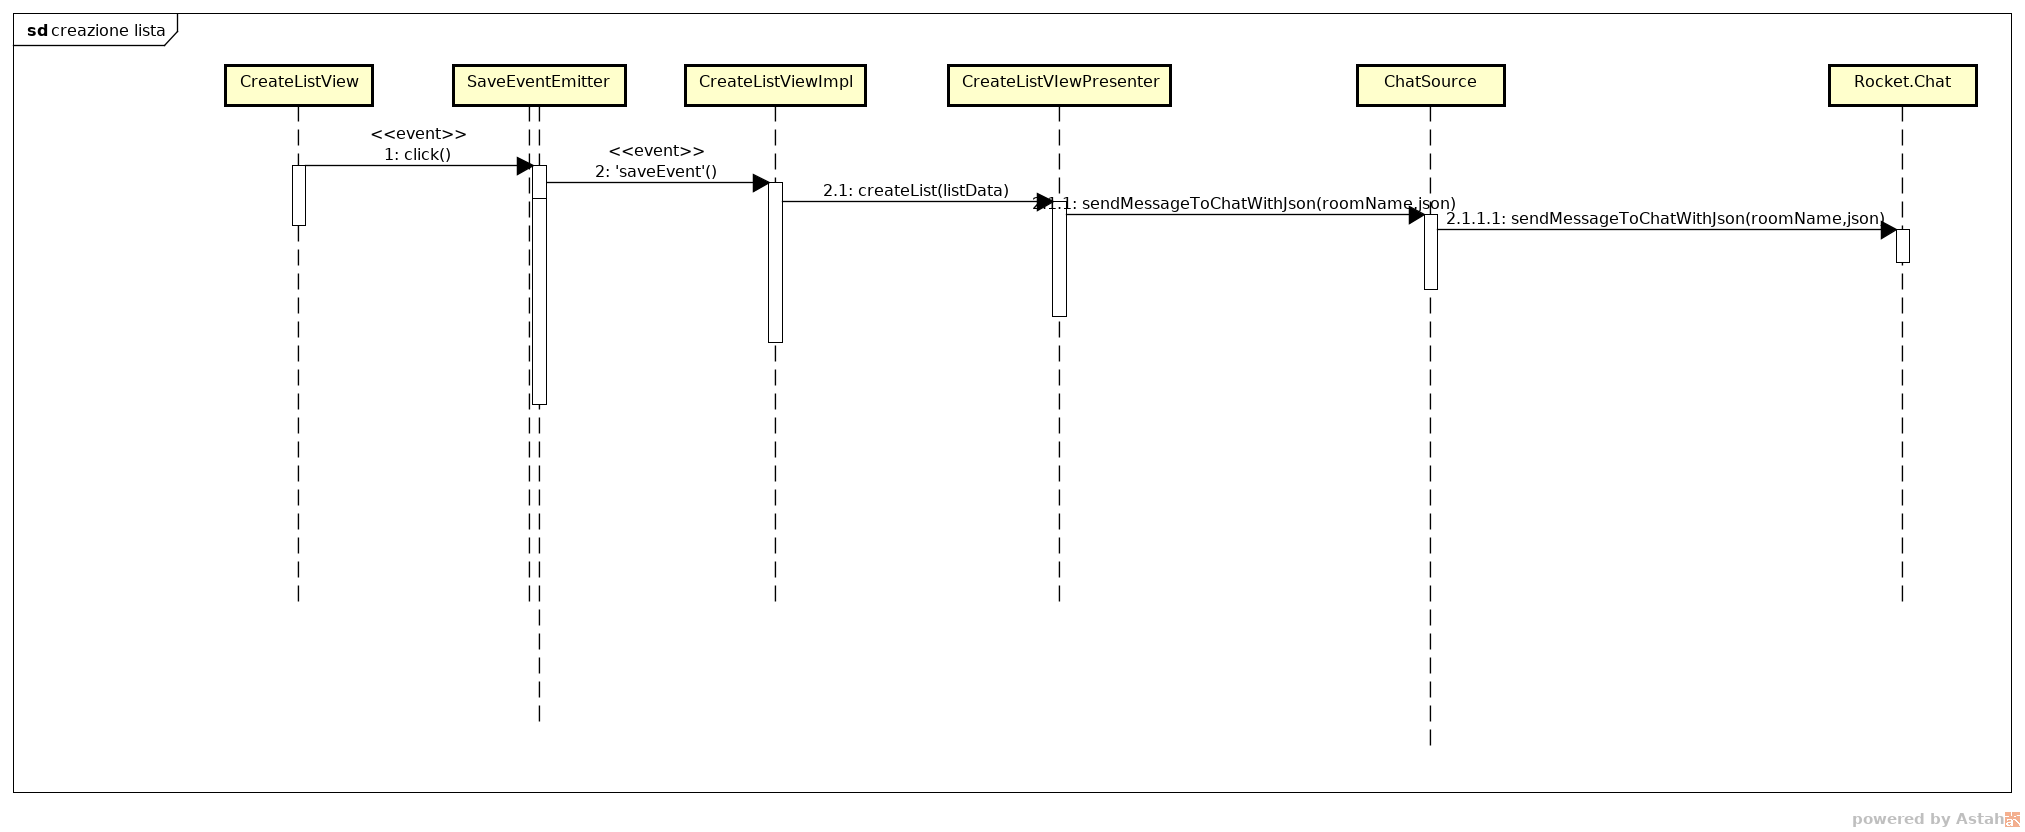
\includegraphics[ width=\textwidth]{Sezioni/Diagrammi/App/creazionelista.png}
	\caption{Creazione di una lista}
\end{figure}

Questo scenario rappresenta l'utente che vuole creare una nuova lista nella chat di \termine{Rocket.chat}. Innanzitutto alla pressione del pulsante creazione lista verrà emesso un evento che verrà catturato dalla classe \textit{InputListInfoView} che incapsulerà i dati della lista e demanderà la gestione di essi al presenter. Quest'ultimo emetterà un evento di tipo \textit{'saveEvent'}, che verrà catturato da \textit{CreateListView}, che demanderà al presenter la creazione vera e propria della lista; quest'ultimo infatti si occuperà di contattare \textit{ChatSource} che farà visualizzare la lista su Rocket.Chat.



\subsubsection{Cancellazione di una lista}

\label{Cancellazione di una lista}
\begin{figure}[H]
	\centering
	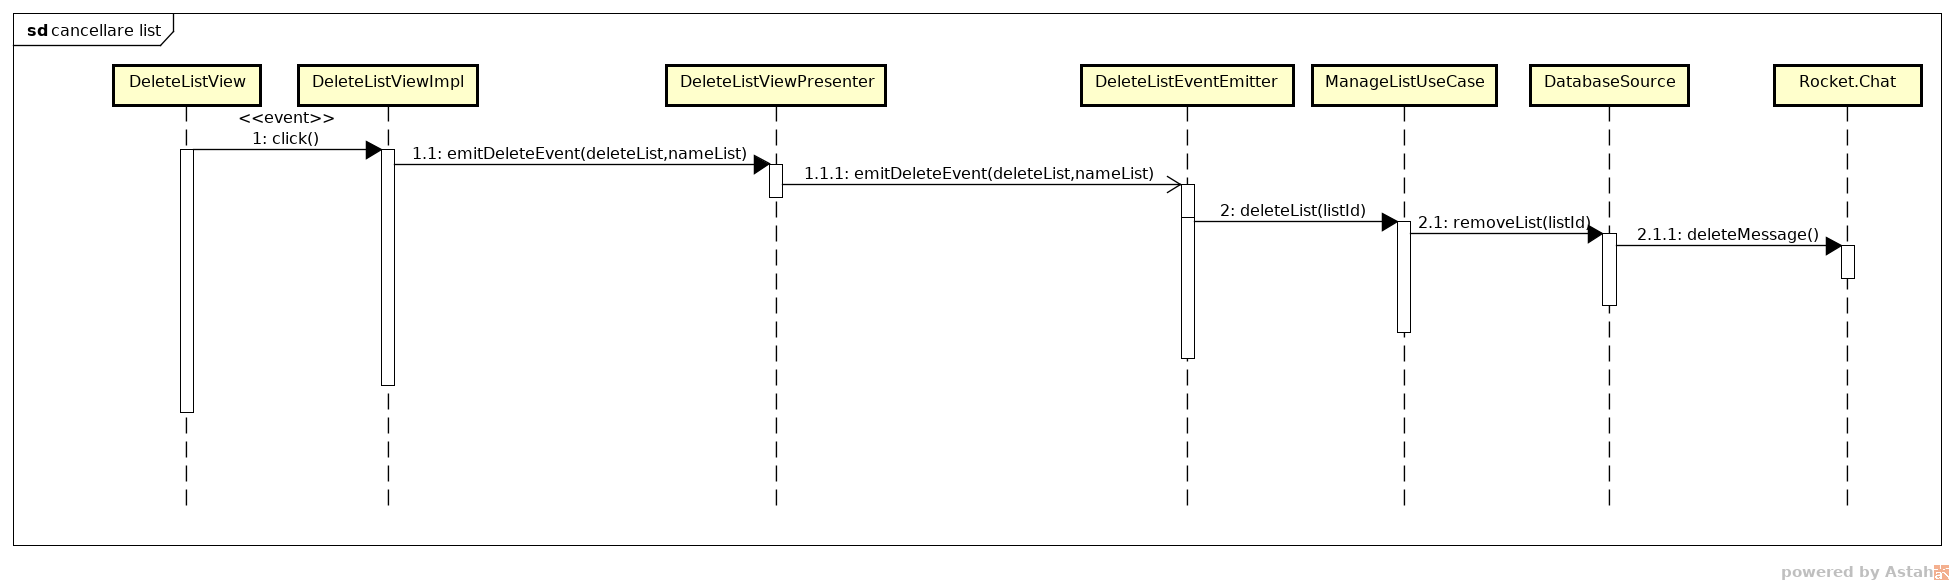
\includegraphics[width=\textwidth]{Sezioni/Diagrammi/App/cancellarelist.png}
	\caption{Cancellazione di una lista}
\end{figure}

In questo scenario lo sviluppatore vuole cancellare la propria lista causandone l'eliminazione da tutte le chat che la contengono. L'utente quando premerà il bottone "Elimina lista" farà emettere un evento di tipo \textit{DeleteEvent}, che verrà catturato da \textit{DeleteListView}, che demanderà al presenter la gestione dell'eliminazione; quest'ultimo userà infatti \textit{ManageListUseCase} per comunicare a \textit{DataBaseSource} che la lista venga eliminata.

\subsubsection{Spunta di un oggetto della lista}

\label{Spunta di un oggetto della lista}
\begin{figure}[H]
	\centering
	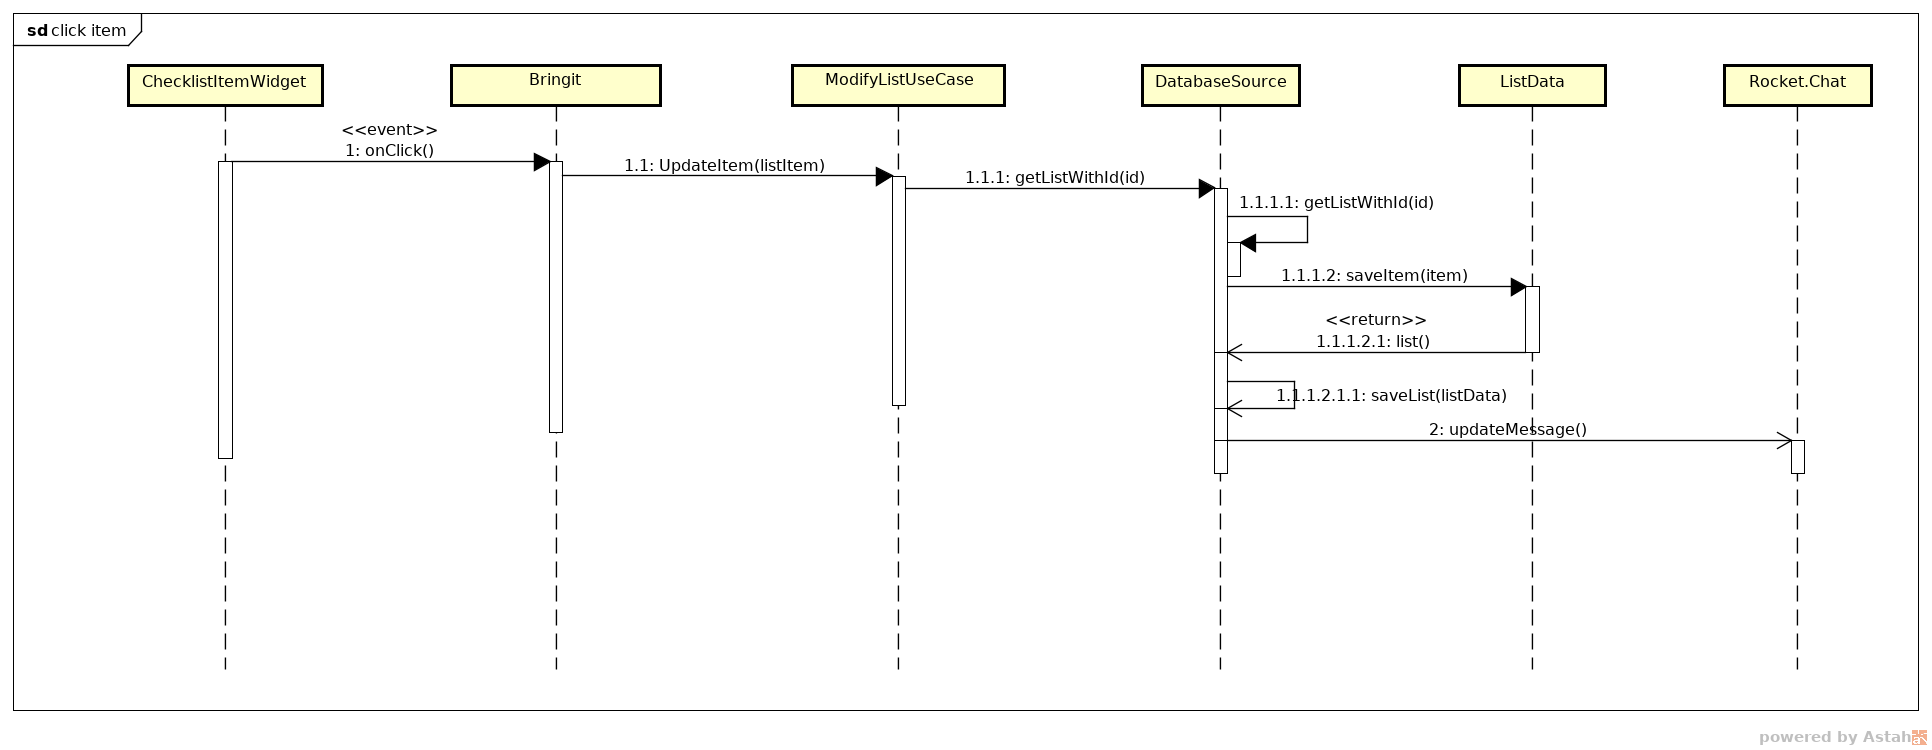
\includegraphics[width=\textwidth]{Sezioni/Diagrammi/App/clickitem.png}
	\caption{Interaione con lista}
\end{figure}

In questo scenario l'utente vuole spuntare un oggetto per segnarlo come \textit{acquistato}.
Per farlo l'utente clicca sul segno del quadrato: questo scatena l'evento del widget \textit{ChecklistItemWidget}, che viene catturato dalla lista \textit{Bringit}, la quale cambia la visualizzazione della lista in \termine{Rocket.Chat} e attraverso \textit{ModifyListUseCase} fa si che la modifica di stato avvenuta venga applicata anche alla permanenza dei dati grazie a \textit{DatabaseSource}.


\subsubsection{Aggiunta di un Item}

\label{Aggiunta di un Item}
\begin{figure}[H]
	\centering
	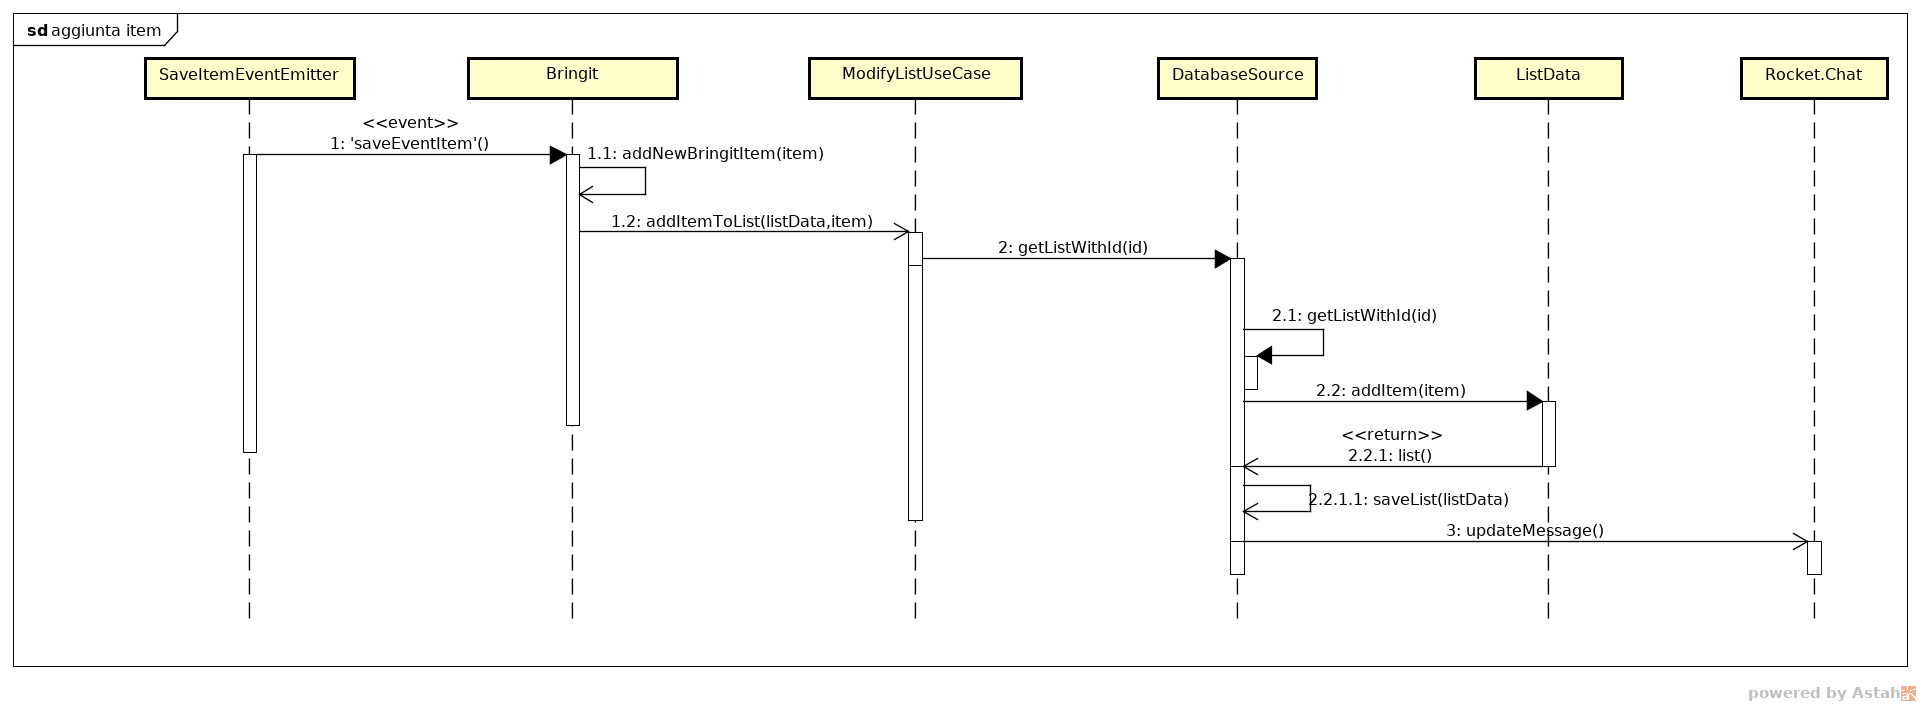
\includegraphics[width=\textwidth]{Sezioni/Diagrammi/App/aggiuntaitem.png}
	\caption{Aggiunta di un Item}
\end{figure}

In questo scenario lo sviluppatore vuole aggiungere dei prodotti (chiamati item nella nostra applicazione) alla lista da esso creata. Oppure vuole aggiungerli a una lista nella quale ha permessi di modifica. L'utente premendo il pulsante \textit{aggiungi item} farà emettere un evento che verrà catturato dalla classe \textit{Bringit}, che aggiungerà il nuovo item a se stessa e attraverso l'uso di \textit{ModifyListUseCase} fa si che l'aggiunta dell'item avvenuta venga applicata anche alla permanenza dei dati grazie a \textit{DatabaseSource}.


\subsubsection{Modifica Item}

\label{Modifica Item}
\begin{figure}[H]
	\centering
	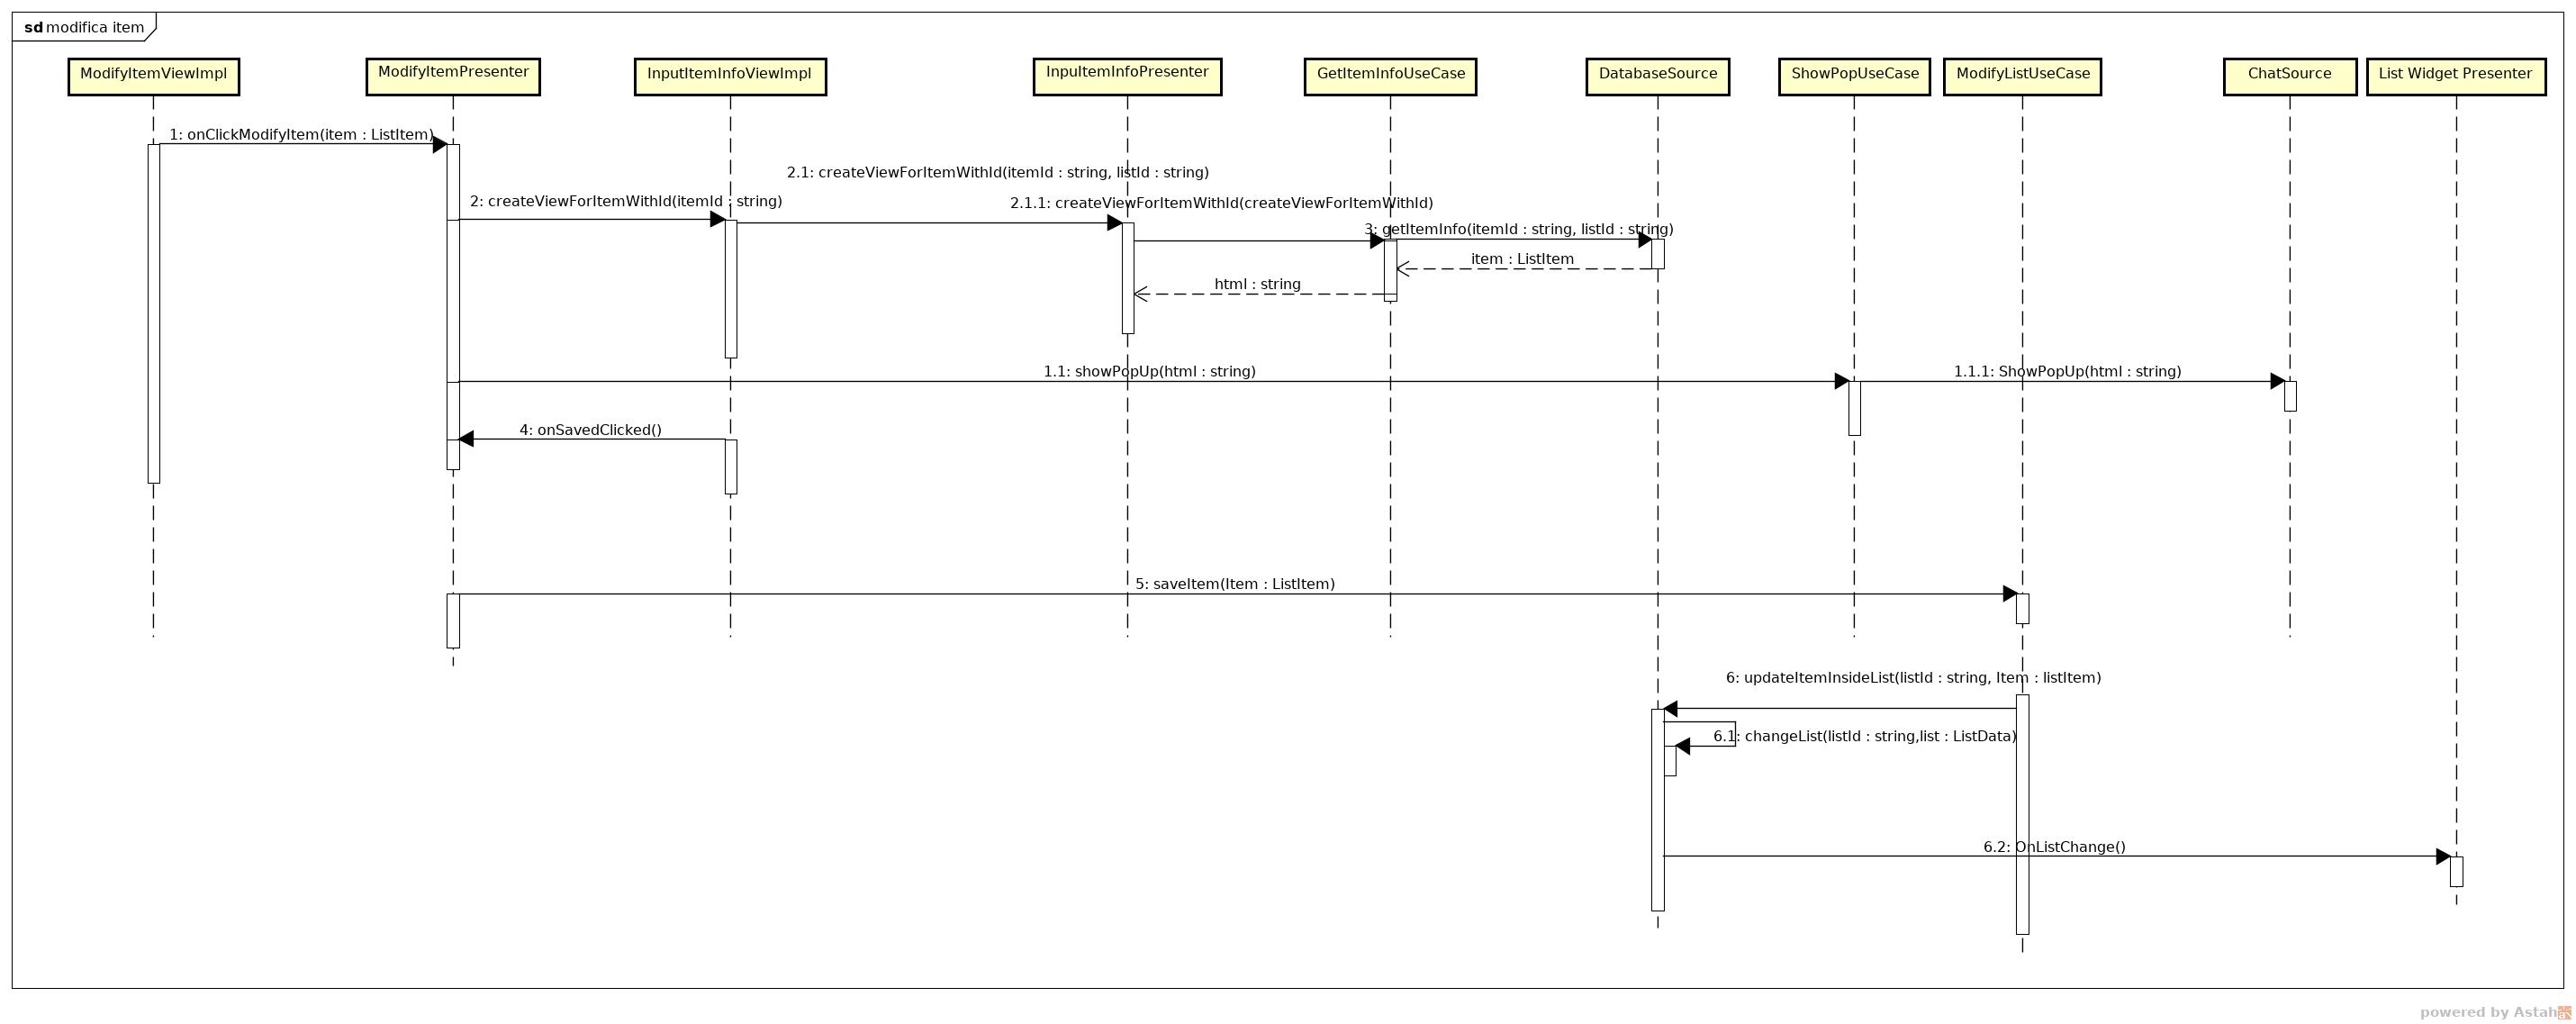
\includegraphics[width=\textwidth]{Sezioni/Diagrammi/App/modifica_item.jpg}
	\caption{Modifica Item}
\end{figure}

In questo scenario lo sviluppatore vuole modificare le informazioni di un item già presente nella lista. L'utente premendo il bottone per la modifica di un item attiverà l'emissione di un evento che verrà catturato dalla classe \textit{ModifyItemViewImpl} demandando la gestione al suo presenter. Quest'ultimo attraverso il suo metodo \textit{createViewForItemWithId} gli ritornerà l'HTML per la creazione della vista dedita alla modifica dell'item con i campi dati precompilati utilizzando le informazioni contenute nel \termine{database}. Successivamente richiamando il metodo \textit{showPopUp} l'utente visualizzerà a schermo le informazioni prima ottenute con la possibilità di modifica. Una volta modificate le informazioni desiderate l'utente premerà il pulsante di conferma modifica, verrà quindi emesso l'evento di salvataggio che verrà catturato dalla classe \textit{InputItemInfoViewImpl} e successivamente demandato a \textit{ModifyItemPresenter} che si occuperà di salvare le modifiche effettuate nel \termine{database}. Infine all'avvenuta modifica della lista nel \termine{database} verranno eseguiti i metodi nel presenter della bolla lista per aggiornare tutte le chat contenenti l'istanza della lista appena modificata. 

\subsubsection{Rimozione Item}

\label{Rimozione Item }
\begin{figure}[H]
	\centering
	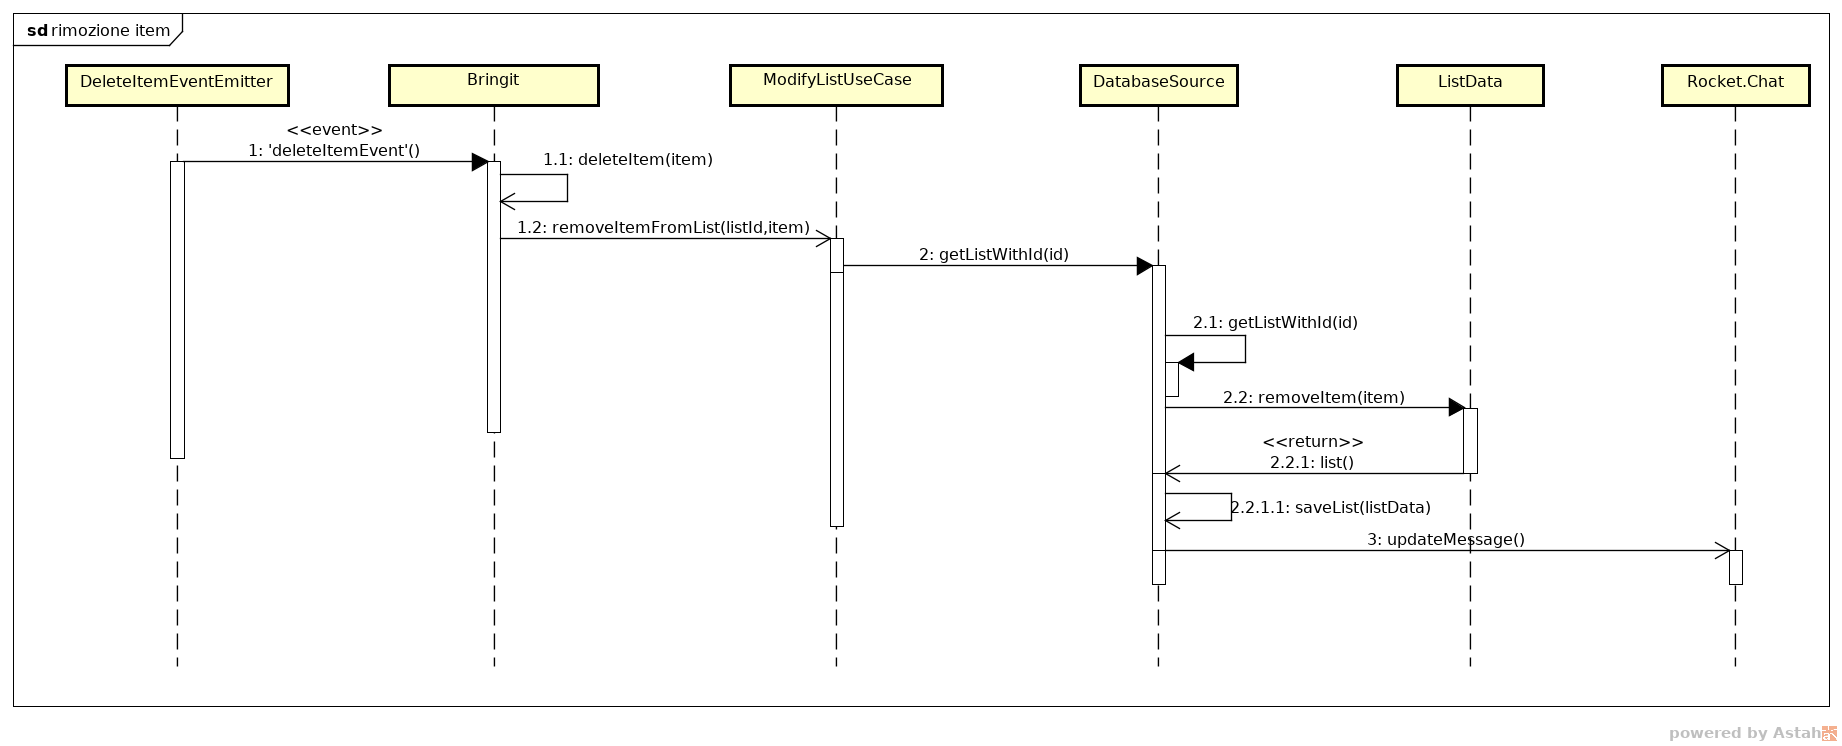
\includegraphics[width=\textwidth]{Sezioni/Diagrammi/App/rimozioneitem.png}
	\caption{Rimozione Item}
	
\end{figure}
In questo scenario l'utente vuole eliminare un item dalla lista. Per farlo l'utente deve premere il pulsante rimuovi item attivando quindi un evento che verrà catturato dalla classe \textit{Bringit}, che analogamente a quanto fa per l'aggiunta di un item, rimuove la parte grafica dell'item che si è deciso di eliminare e utilizza \textit{ModifyListUseCase} e \textit{DatabaseSource} per salvare le modifiche effettuate alla lista Bringit.


\subsubsection{Pubblicazione a un contatto}

\label{Pubblicazione di un contatto}
\begin{figure}[H]
	\centering
	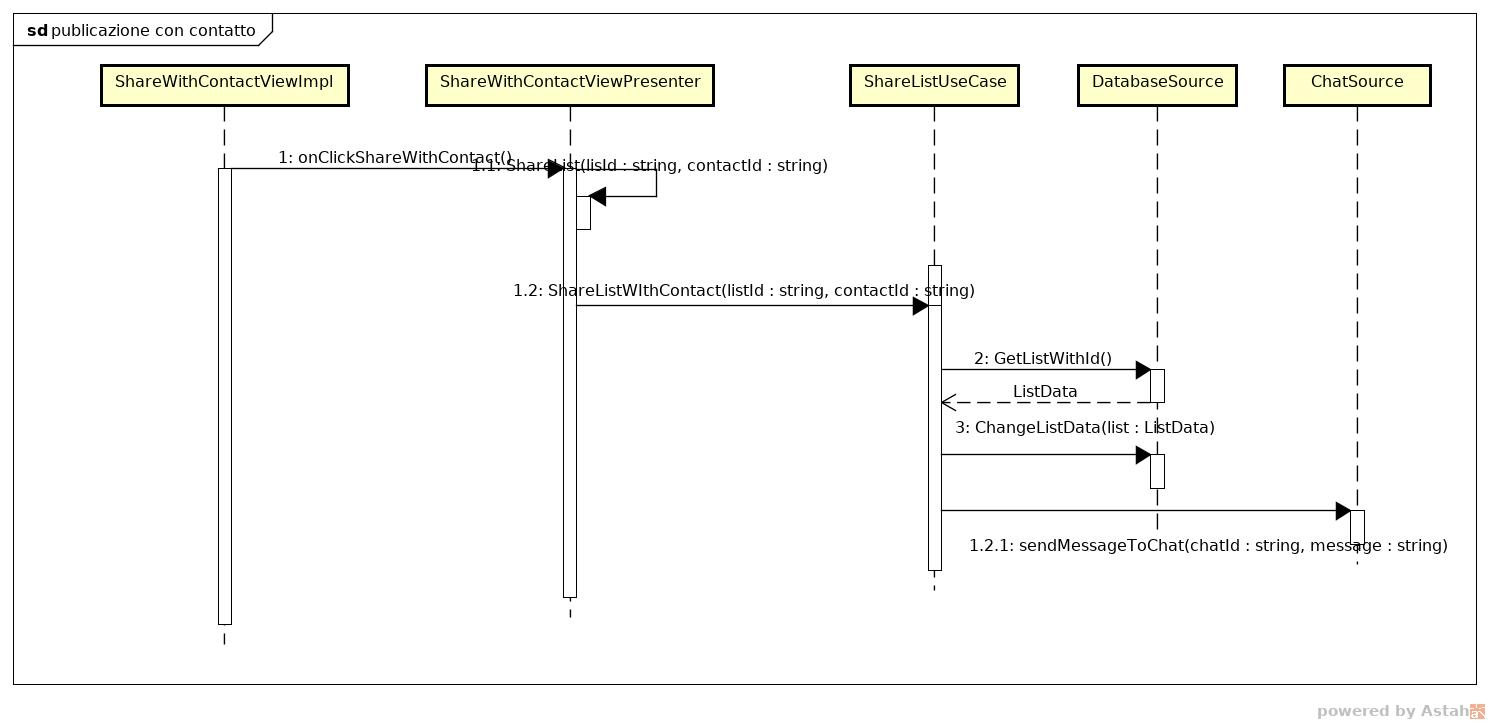
\includegraphics[width=\textwidth]{Sezioni/Diagrammi/App/publicazione_con_contatto.jpg}
	\caption{Pubblicazione di un contatto}
	
\end{figure}
In questo scenario l'utente vuole pubblicare la lista ad un altro contatto, dando il permesso di modifica e interazione con la lista. L'utente premendo il bottone \textit{pubblica lista} sceglierà un contatto, lanciando quindi un evento che verrà catturato dalla classe \textit{ShareWithContactViewImpl} e demandato al suo presenter che, tramite il metodo \textit{shareList}, attiverà i metodi utili per aggiungere i permessi necessari al interazione al utente scelto. Successivamente la classe \textit{ShareListUseCase} si occuperà di salvare le modifiche nel \termine{database} e pubblicare infine all'utente desiderato la lista tramite il metodo {sendMessageToChat}.


\subsubsection{Pubblicazione a un gruppo}

\label{Pubblicazione a un gruppo}
\begin{figure}[H]
	\centering
	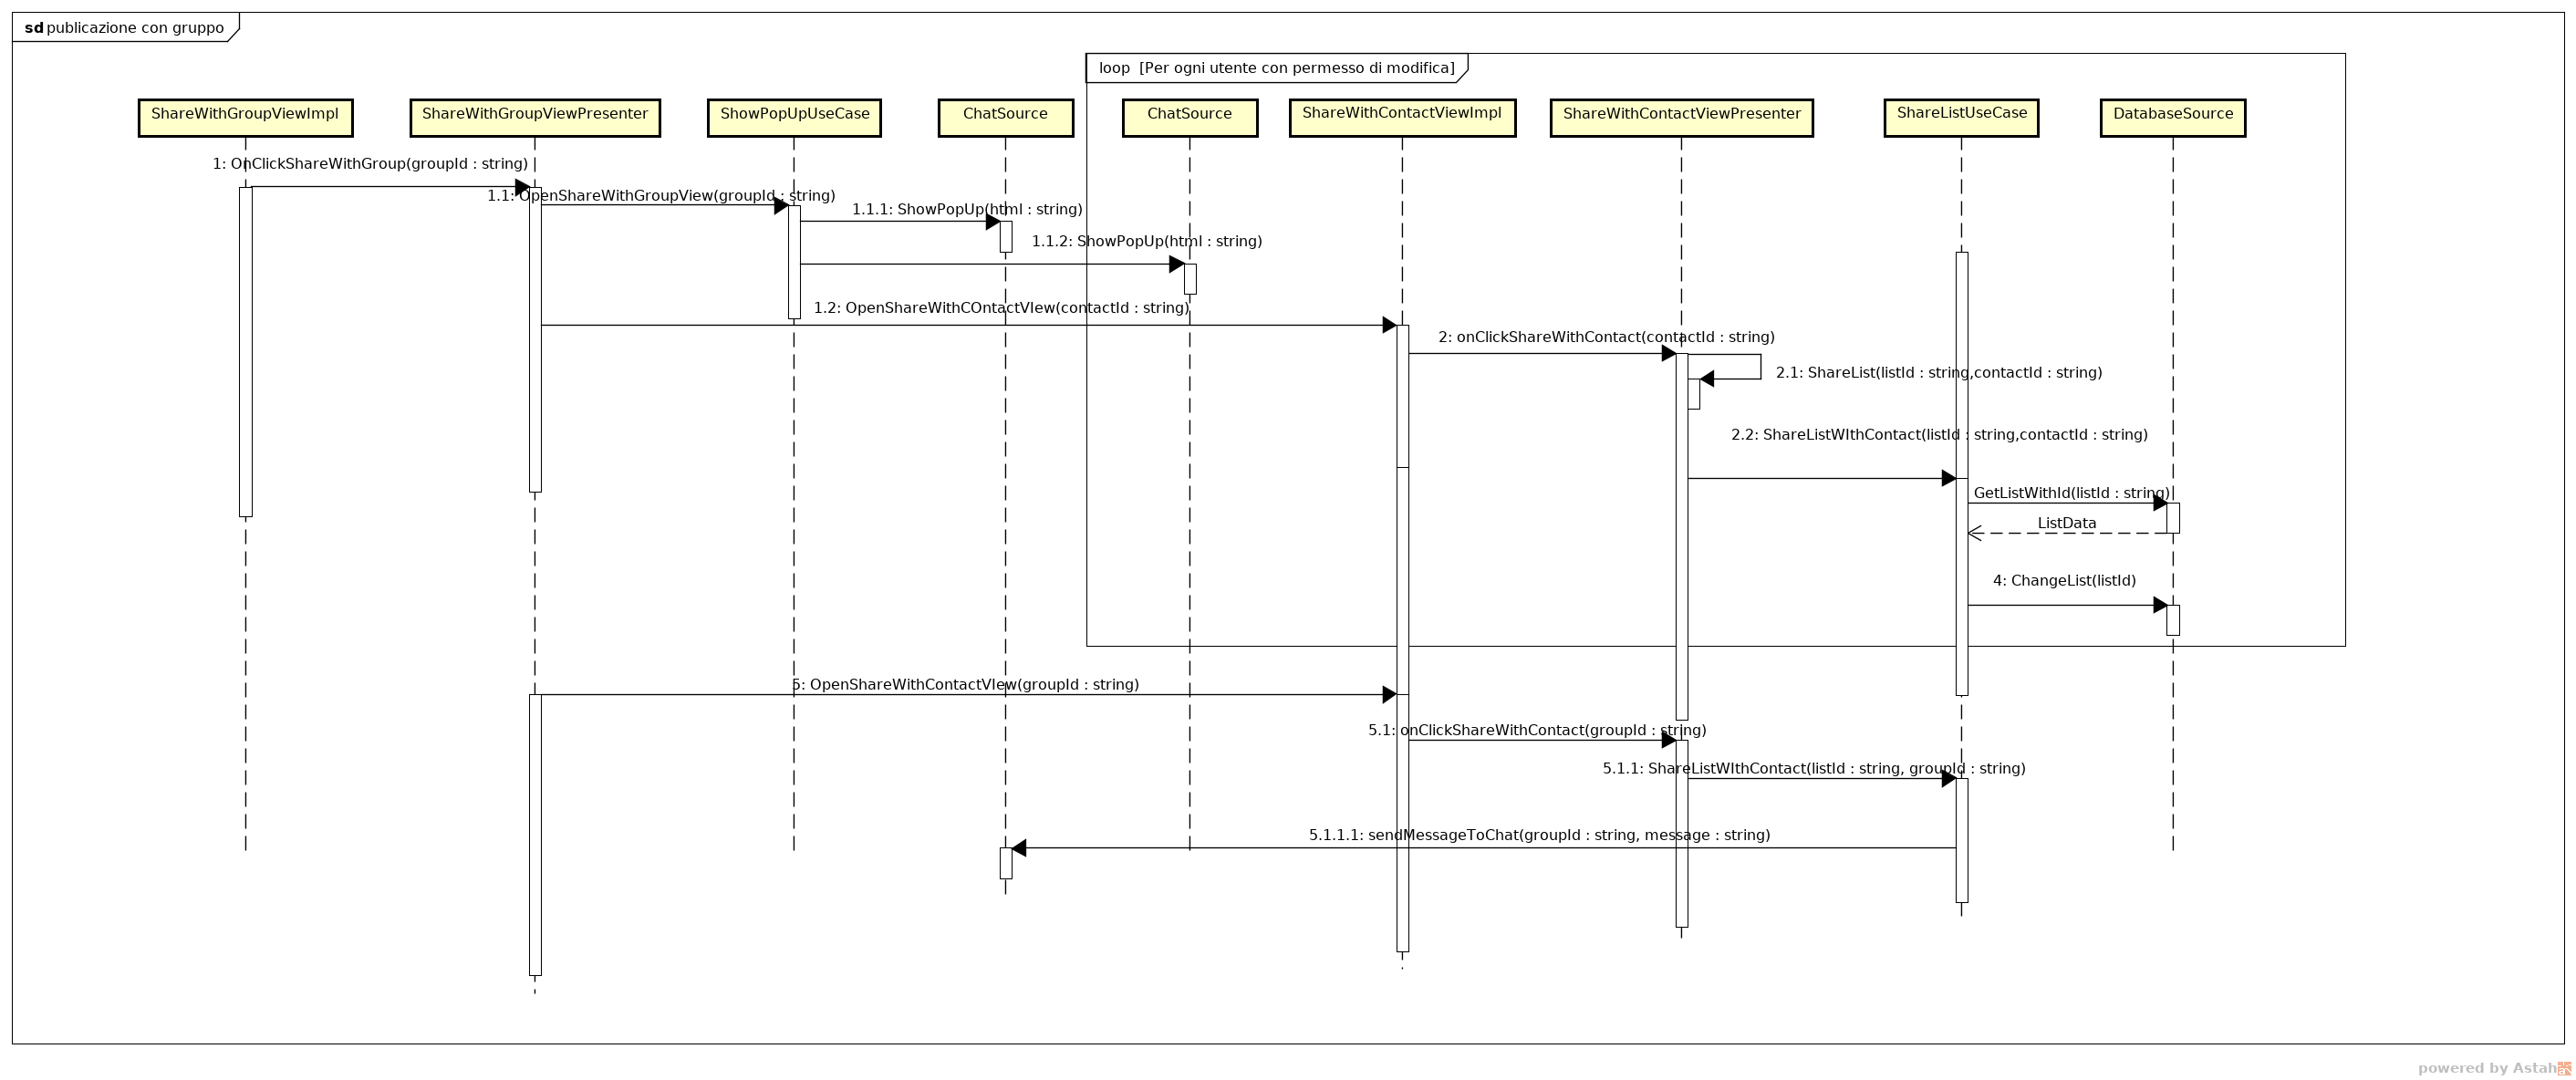
\includegraphics[width=\textwidth]{Sezioni/Diagrammi/App/publicazionecongruppo.png}
	\caption{Pubblicazione a un gruppo}
	
\end{figure}

Simile allo scenario precedente in questo caso l'utente vuole condividere e dare i permessi ad utenti specifici presenti all'interno di un gruppo. L'utente premendo il bottone \textit{pubblica lista} sceglierà un gruppo, lanciando quindi un evento che verrà catturato dalla classe \textit{ShareWithGroupViewImpl} e demanderà la gestione al suo presenter. Quest'ultimo attraverso il metodo \textit{openShareWithGroup} inizializzerà un ciclo che porterà a scegliere per ogni utente presente nel gruppo la concessione o meno dei permessi. La procedura per svolgere il ruolo sopra descritto è simile allo scenario della \textit{pubblicazione con contatto} con la differenza che non verrà inviato un messaggio agli utenti con i permessi concessi. Infine terminato il ciclo verrà si passerà per \textit{ShareListUseCase}, che si occuperà di salvare le modifiche apportate alla lista nel database.

\subsubsection{Inoltro a un contatto}

\label{Inoltro a un contatto}
\begin{figure}[H]
	\centering
	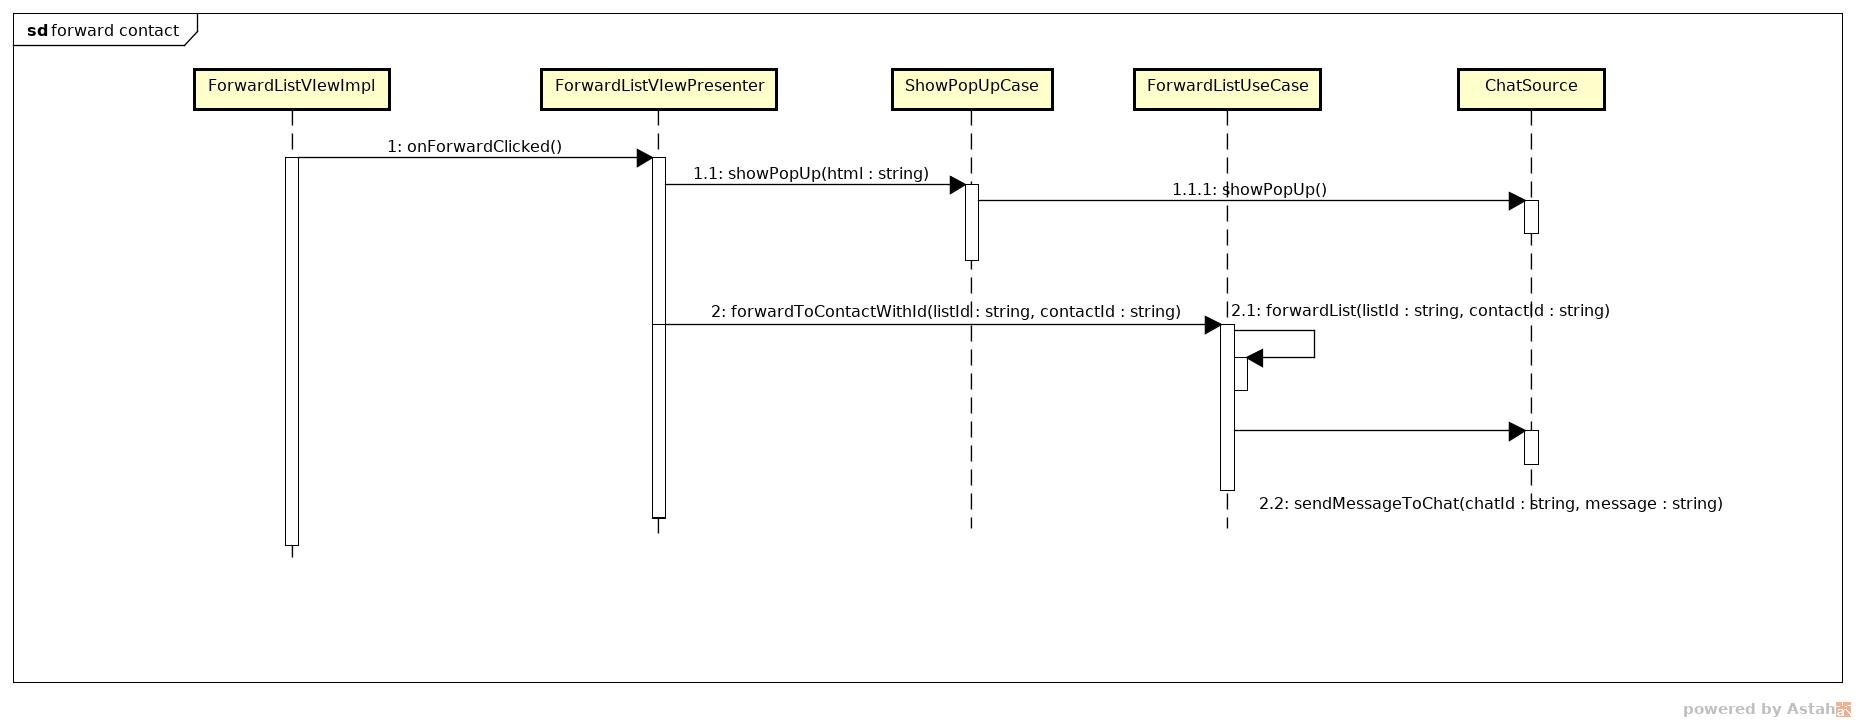
\includegraphics[width=\textwidth]{Sezioni/Diagrammi/App/forward_contatto.jpg}
	\caption{Inoltro a un contatto}
	
\end{figure}

In questo scenario l'utente vuole inoltrare la lista ad un contatto come fosse un semplice messaggio di testo, senza aggiungere allo specifico contatto nessun permesso di modifica o interazione. L'utente premendo il bottone di inoltro sceglierà un contatto. Si verificherà quindi l'evento che verrà catturato dalla classe \textit{ForwardListViewImpl} demandandone la gestione al suo presenter.
Quest'ultimo con il metodo \textit{forwardToContactWithId} inoltrerà la lista al contatto desiderato attraverso la classe \textit{ChatSource}. Prima dell'avvenuto inoltro al contatto selezionato verrà chiamato il metodo \textit{showPopUp} che, interfacciandosi con la classe \textit{ForwardListUseCase}, mostrerà a schermo un messaggio di conferma per l'inoltro e la scelta per il contatto a cui inoltrare il messaggio.



\subsubsection{Inoltro a un gruppo}

\label{Inoltro a un contatto}
\begin{figure}[H]
	\centering
	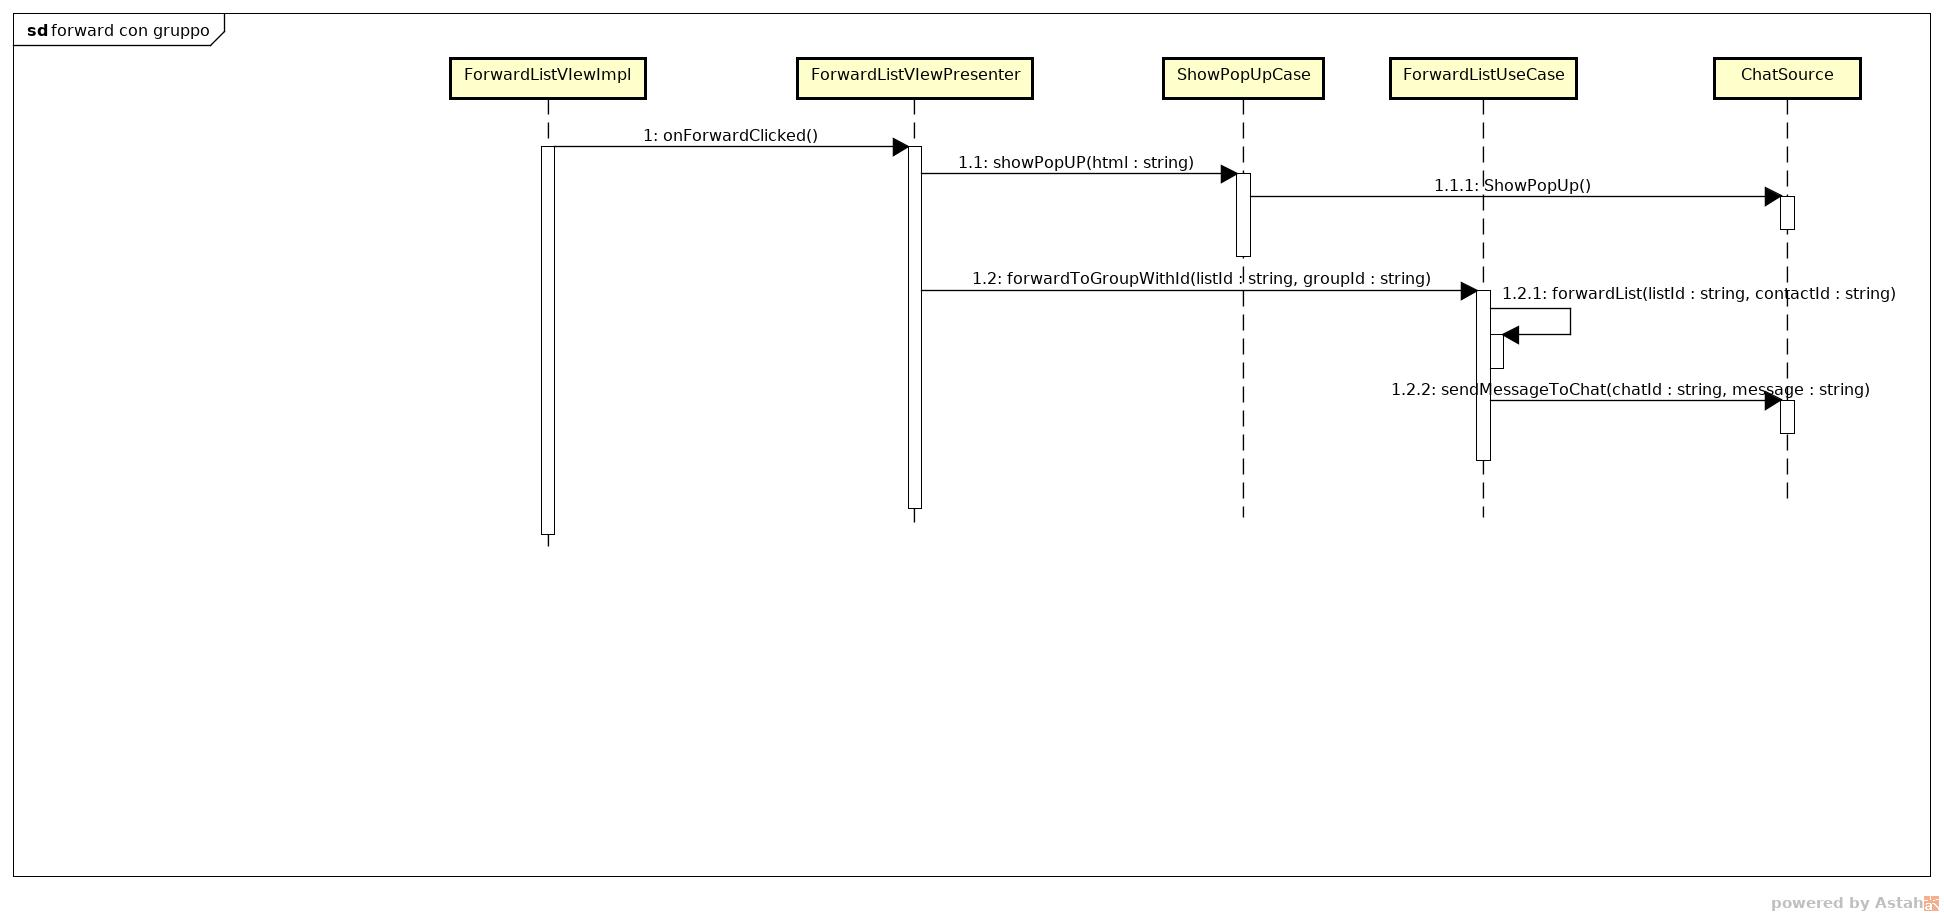
\includegraphics[width=\textwidth]{Sezioni/Diagrammi/App/forward_con_gruppo.jpg}
	\caption{Inoltro a un contatto}
	
\end{figure}

In questo scenario l'utente vuole inoltrare la lista ad un gruppo come fosse un semplice messaggio di testo, senza aggiungere al specifico gruppo nessun permesso di modifica o interazione. L'utente premendo il bottone di inoltro sceglierà un gruppo. Si verificherà quindi l'evento che verrà catturato dalla classe \textit{ForwardListViewImpl} demandandone la gestione al suo presenter.
Quest'ultimo con il metodo \textit{forwardToGroupWithId} inoltrerà la lista al gruppo desiderato attraverso la classe \textit{ChatSource}. Prima dell'avvenuto inoltro al gruppo verrà chiamato il metodo \textit{showPopUp} che, interfacciandosi con la classe \textit{ForwardListUseCase}, mostrerà a schermo un messaggio di conferma per l'inoltro e la selezione del gruppo a cui si desidera inoltrare.


\subsubsection{Help}

\label{Help}
\begin{figure}[H]
	\centering
	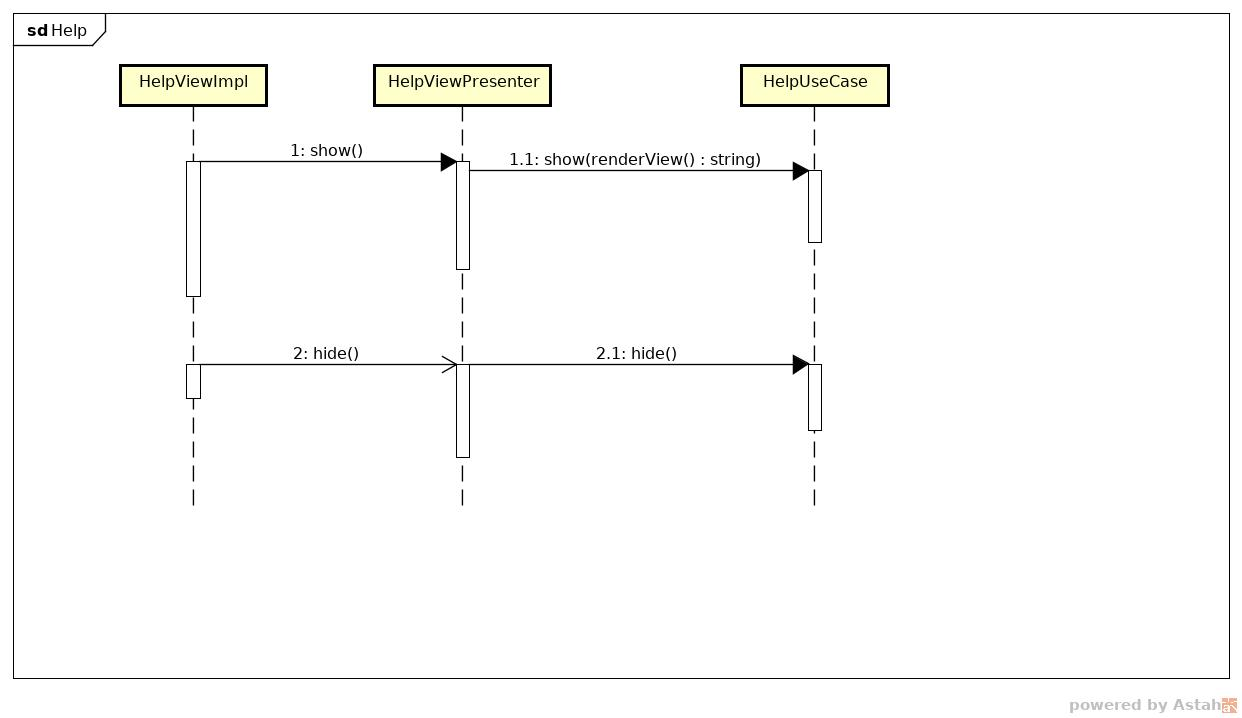
\includegraphics[width=\textwidth]{Sezioni/Diagrammi/App/Help.jpg}
	\caption{Help}
	
\end{figure}

In questo scenario l'utente vuole chiedere delle informazioni d'aiuto per l'utilizzo della nostra applicazione. Per richiedere aiuto l'utente dovrà cliccare il bottone di help apposito. In questa maniera verrà attivato un metodo nella classe \textit{HelpViewImpl} che demanderà la gestione al suo presenter. Quest'ultimo attraverso il metodo \textit{show} farà visualizzare a schermo un popup con le informazioni utili. Per nascondere le informazioni d'aiuto avremo lo stesso flusso di utilizzo con il metodo \textit{hide} in sostituzione al metodo \textit{show} attivabile nella stessa maniera.
